\documentclass[a4paper,12pt]{article}
\usepackage{xcolor}
\usepackage{amsmath,amsfonts,amssymb}
\usepackage{geometry}
\usepackage{fancyhdr}
\usepackage{graphicx}
\usepackage{subcaption} % For subfigure support
\usepackage{float} % For [H] placement
\usepackage{titlesec}
\usepackage{tikz}
\usepackage{booktabs}
\usepackage{array}
\usetikzlibrary{shadows}
\usepackage{tcolorbox}
\usepackage{float}
\usepackage{lipsum}
\usepackage{mdframed}
\usepackage{pagecolor}
\usepackage{mathpazo}   % Palatino font (serif)
\usepackage{microtype}  % Better typography

% Page background color
\pagecolor{gray!10!white}

% Geometry settings
\geometry{margin=0.5in}
\pagestyle{fancy}
\fancyhf{}

% Fancy header and footer
\fancyhead[C]{\textbf{\color{blue!80}CS754 Assignment-1}}
% \fancyhead[R]{\color{blue!80}Saksham Rathi}
\fancyfoot[C]{\thepage}

% Custom Section Color and Format with Sans-serif font
\titleformat{\section}
{\sffamily\color{purple!90!black}\normalfont\Large\bfseries}
{\thesection}{1em}{}

% Custom subsection format
\titleformat{\subsection}
{\sffamily\color{cyan!80!black}\normalfont\large\bfseries}
{\thesubsection}{1em}{}

% Stylish Title with TikZ (Enhanced with gradient)
\newcommand{\cooltitle}[1]{%
  \begin{tikzpicture}
    \node[fill=blue!20,rounded corners=10pt,inner sep=12pt, drop shadow, top color=blue!50, bottom color=blue!30] (box)
    {\Huge \bfseries \color{black} #1};
  \end{tikzpicture}
}
\usepackage{float} % Add this package

\newenvironment{solution}[2][]{%
    \begin{mdframed}[linecolor=blue!70!black, linewidth=2pt, roundcorner=10pt, backgroundcolor=yellow!10!white, skipabove=12pt, skipbelow=12pt]%
        \textbf{\large #2}
        \par\noindent\rule{\textwidth}{0.4pt}
}{
    \end{mdframed}
}

% Document title
\title{\cooltitle{CS754 Assignment-1}}
\author{{\bf Saksham Rathi, Ekansh Ravi Shankar, Kshitij Vaidya}}
\date{}

\begin{document}
\maketitle

\textbf{Declaration:} The work submitted is our own, and
we have adhered to the principles of academic honesty while completing and submitting this work. We have not referred to any unauthorized sources, and we have not used generative AI tools for the work submitted here.

\section*{Question 5}

\begin{solution}{OMP}
The code is present in the file \texttt{assignment1/5/code/omp.m}. On opening matlab in that folder, the code can be run by executing the command \texttt{omp}.

Firstly, we need to plot RMSE vs m (number of measurements), for various values of sparsity $k$. 

\begin{figure}[H]
  \centering
  % First subfigure
  \begin{subfigure}[t]{0.32\textwidth}
      \centering
      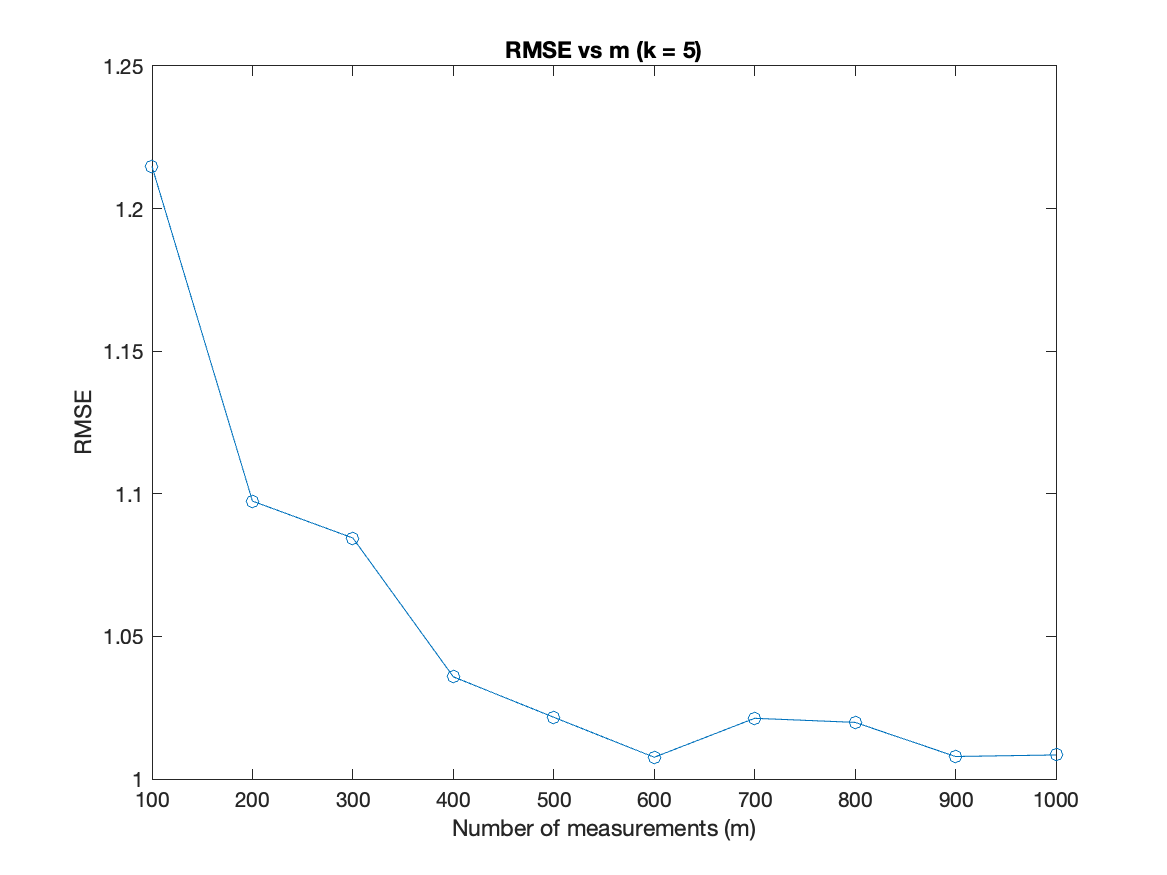
\includegraphics[width=\textwidth]{../images/omp/RMSE_vs_m_k_5.png}
      \caption{RMSE vs m for $k = 5$}
  \end{subfigure}
  % Second subfigure
  \begin{subfigure}[t]{0.32\textwidth}
      \centering
      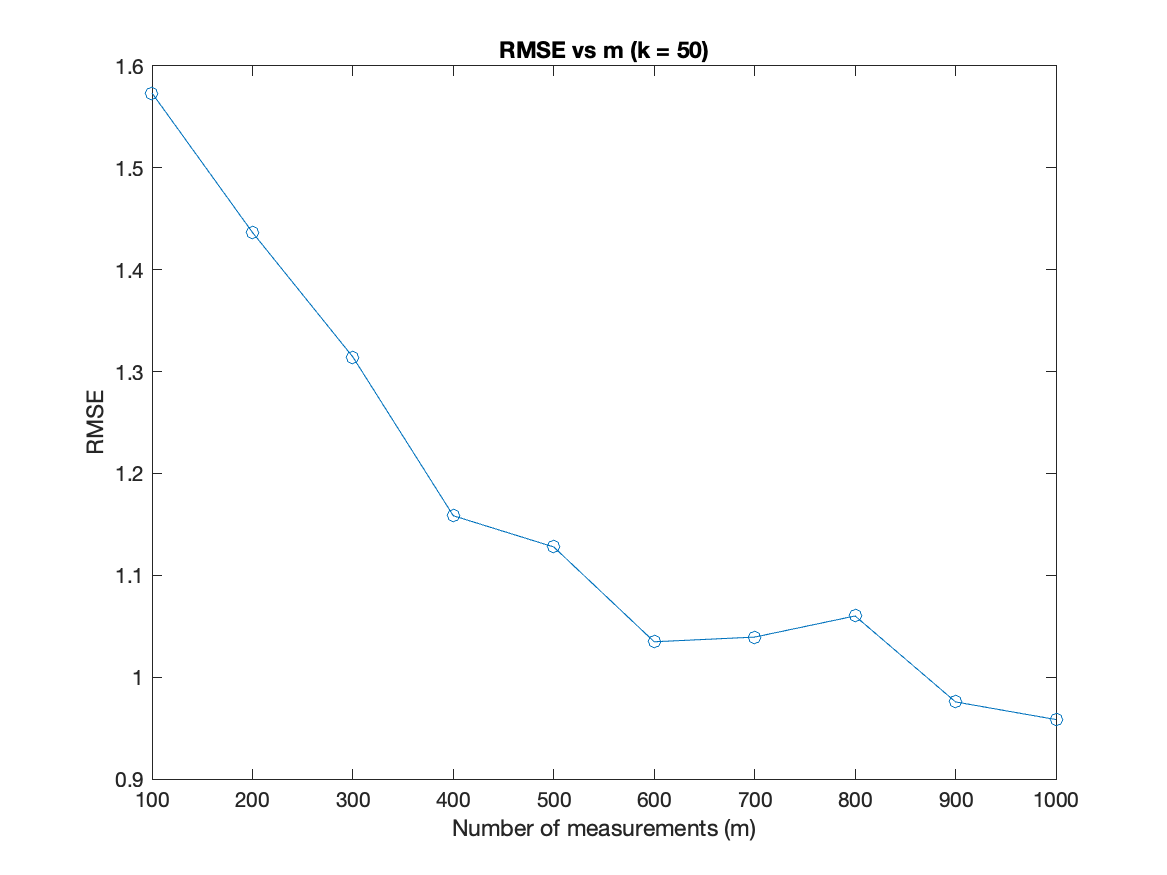
\includegraphics[width=\textwidth]{../images/omp/RMSE_vs_m_k_50.png}
      \caption{RMSE vs m for $k = 50$}
  \end{subfigure}
  % Third subfigure
  \begin{subfigure}[t]{0.32\textwidth}
      \centering
      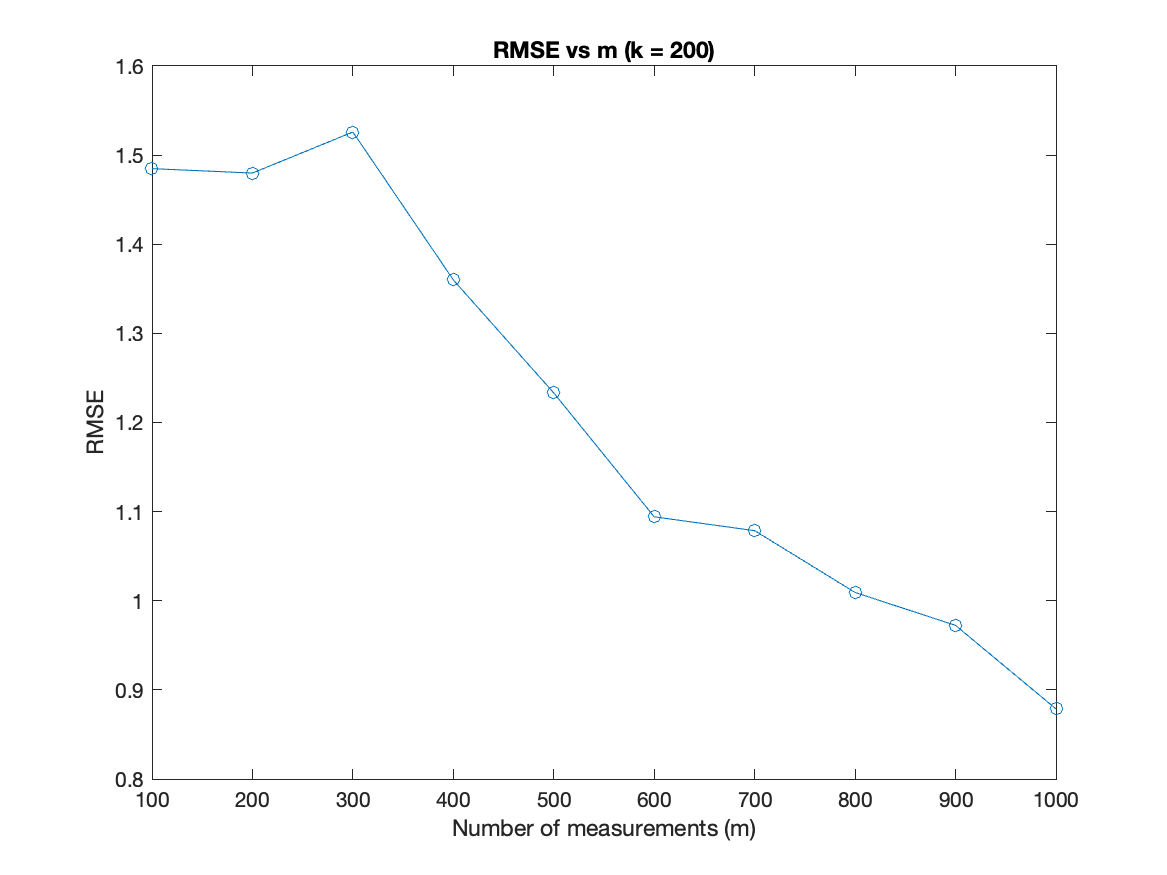
\includegraphics[width=\textwidth]{../images/omp/RMSE_vs_m_k_200.png}
      \caption{RMSE vs m for $k = 200$}
  \end{subfigure}
  \caption{Comparison of RMSE vs m for different values of $k$ for OMP}
  \label{fig:rmse_comparison}
\end{figure}

From the above plots, we can see that the RMSE decreases as the number of measurements $m$ increases. This is expected, as more measurements provide more information about the signal. Higher $k$ (more nonzero coefficients in the sparse signal) makes reconstruction harder, leading to higher initial RMSE. The performance improvement with $m$ is more gradual for larger $k$, suggesting that a higher number of measurements is needed for accurate recovery when $k$ is large. Small fluctuations in RMSE for intermediate values of $m$ could be due to the randomness in the measurement matrix or noise in the reconstruction.

Next, we plot RMSE vs $k$ for various values of $m$.

\begin{figure}[H]
  \centering
  \begin{subfigure}[t]{0.32\textwidth}
      \centering
      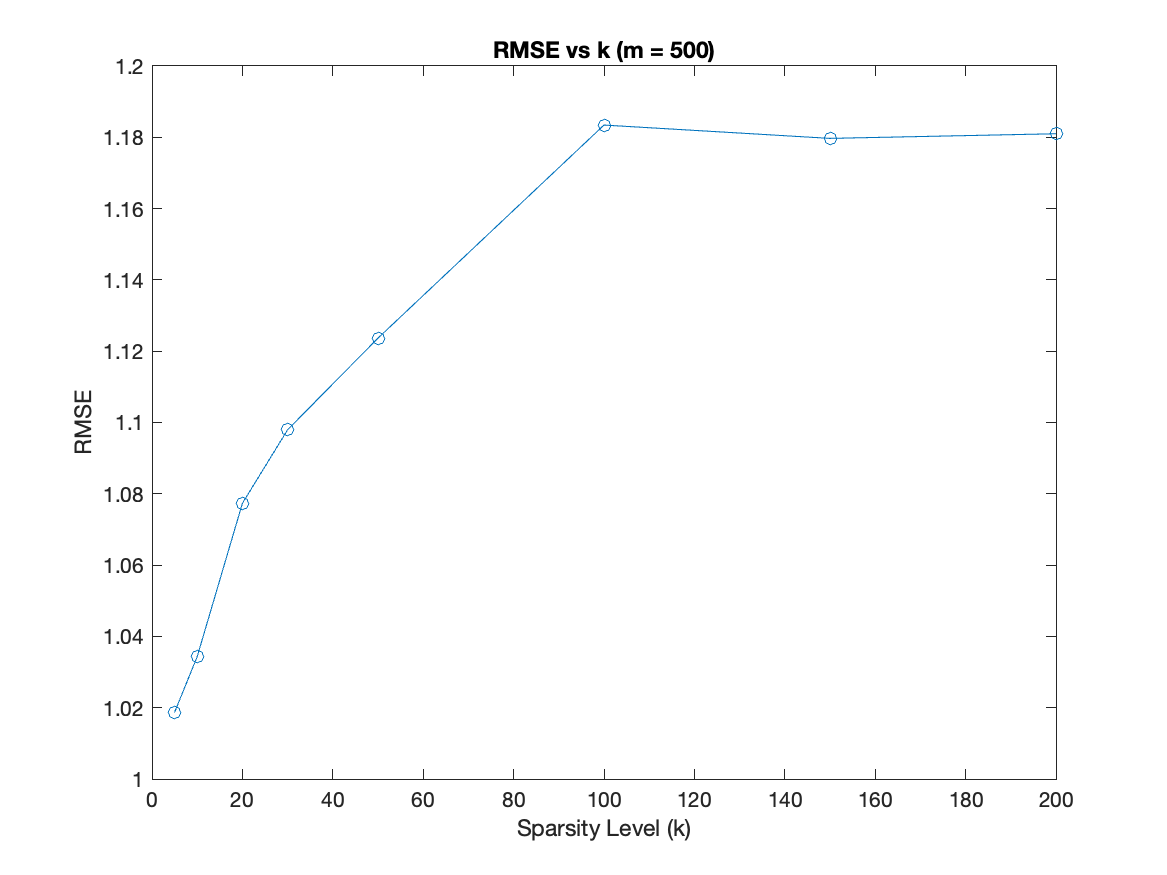
\includegraphics[width=\textwidth]{../images/omp/RMSE_vs_k_m_500.png}
      \caption{RMSE vs k for $m = 500$}
  \end{subfigure}
  \begin{subfigure}[t]{0.32\textwidth}
      \centering
      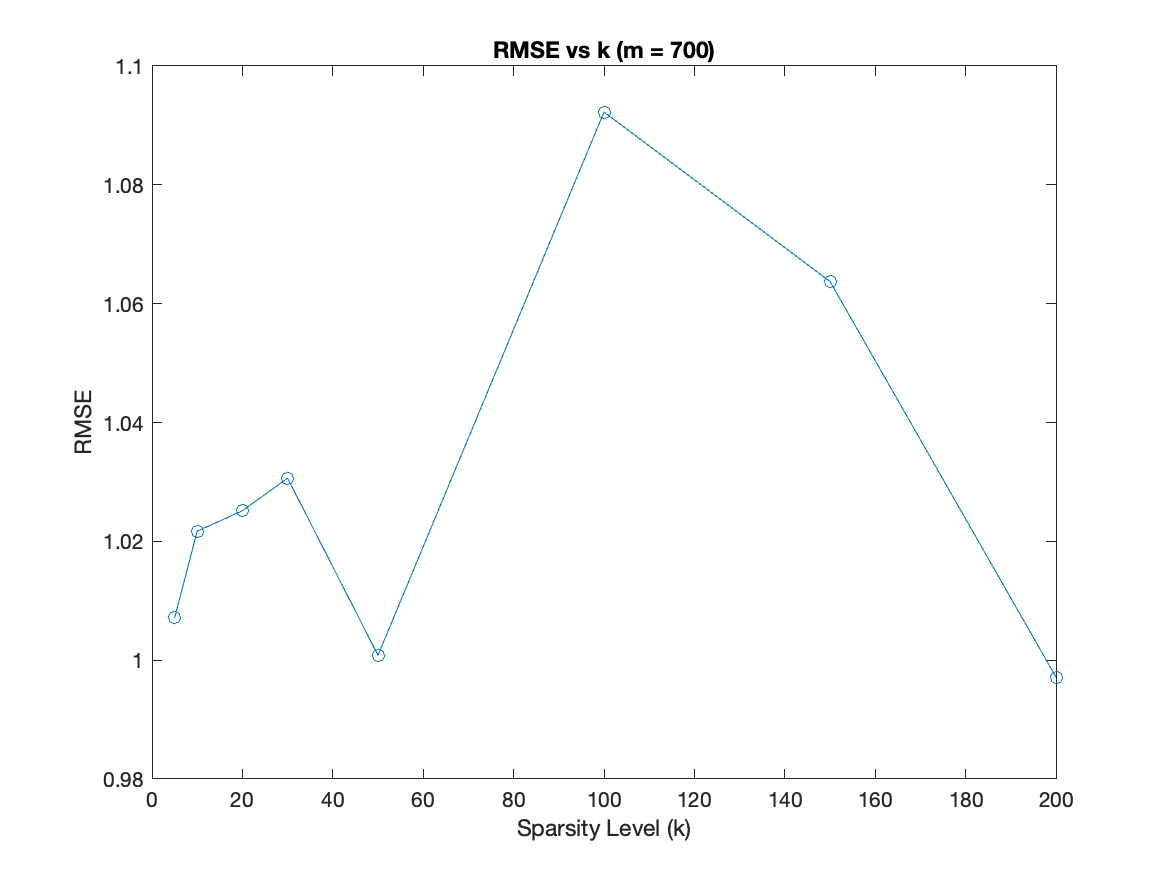
\includegraphics[width=\textwidth]{../images/omp/RMSE_vs_k_m_700.png}
      \caption{RMSE vs k for $m = 700$}
  \end{subfigure}
  \caption{Comparison of RMSE vs k for different values of $m$ for OMP}
  \label{fig:rmse_comparison2}
\end{figure}


In general, as $k$ increases (increase in the number of non-zero indices), the RMSE increases. This is expected, as a higher sparsity level makes reconstruction harder. The RMSE increases more rapidly for smaller $m$, suggesting the better stability incase of larger number of measurements. Some fluctuations in the RMSE for intermediate values of $k$ could be due to the randomness in the measurement matrix or noise in the reconstruction.

Here is the ground truth images for various values of $k$:

\begin{figure}[H]
  \centering
  \begin{subfigure}[t]{0.32\textwidth}
      \centering
      
\includegraphics[width=\textwidth]{../images/omp/Ground_Truth_k_5.png}
      \caption{Ground truth for $k = 5$}
  \end{subfigure}
  \begin{subfigure}[t]{0.32\textwidth}
      \centering
      \includegraphics[width=\textwidth]{../images/omp/Ground_truth_k_50.png}
      \caption{Ground truth for $k = 50$}
  \end{subfigure}
  \begin{subfigure}[t]{0.32\textwidth}
      \centering
      \includegraphics[width=\textwidth]{../images/omp/Ground_truth_k_200.png}
      \caption{Ground truth for $k = 200$}
  \end{subfigure}
  \caption{Ground truth images for different values of $k$}
  \label{fig:ground_truth}
\end{figure}

Here are the corresponding reconstructed images for $m$ values of 500 and 700 (other images can be found in the \texttt{images/omp} folder):

\begin{figure}[H]
  \centering
  % First row
  \begin{subfigure}[t]{0.32\textwidth}
      \centering
      
\includegraphics[width=\textwidth]{../images/omp/Reconstructed_k_5_m_500.png}
      \caption{Reconstructed for $k = 5$, $m = 500$}
  \end{subfigure}
  \begin{subfigure}[t]{0.32\textwidth}
      \centering
      
\includegraphics[width=\textwidth]{../images/omp/Reconstructed_k_5_m_700.png}
      \caption{Reconstructed for $k = 5$, $m = 700$}
  \end{subfigure}
  \begin{subfigure}[t]{0.32\textwidth}
      \centering
      
\includegraphics[width=\textwidth]{../images/omp/Reconstructed_k_50_m_500.png}
      \caption{Reconstructed for $k = 50$, $m = 500$}
  \end{subfigure}

  % Second row
  \begin{subfigure}[t]{0.32\textwidth}
      \centering
      
\includegraphics[width=\textwidth]{../images/omp/Reconstructed_k_50_m_700.png}
      \caption{Reconstructed for $k = 50$, $m = 700$}
  \end{subfigure}
  \begin{subfigure}[t]{0.32\textwidth}
      \centering
      
\includegraphics[width=\textwidth]{../images/omp/Reconstructed_k_200_m_500.png}
      \caption{Reconstructed for $k = 200$, $m = 500$}
  \end{subfigure}
  \begin{subfigure}[t]{0.32\textwidth}
      \centering
      
\includegraphics[width=\textwidth]{../images/omp/Reconstructed_k_200_m_700.png}
      \caption{Reconstructed for $k = 200$, $m = 700$}
  \end{subfigure}

  \caption{Reconstructed images for different values of $k$ and $m$}
  \label{fig:reconstructed_all}
\end{figure}








\end{solution}


\end{document}
